%--------------------------------------------------------------------------
%	PACKAGES AND OTHER DOCUMENT CONFIGURATIONS
%--------------------------------------------------------------------------
\documentclass[12pt,a4paper]{article}
\usepackage[utf8]{inputenc}
\usepackage[francais]{babel}
\usepackage[T1]{fontenc}
\usepackage{amsmath}
\usepackage{amsfonts}
\usepackage{amssymb}
\usepackage{graphicx}
\usepackage{lmodern}
\usepackage[left=2cm,right=2cm,top=2.2cm,bottom=2cm]{geometry}

\usepackage{fancyhdr} % Required for custom headers
\usepackage{lastpage} % Required to determine the last page for the footer
\usepackage{extramarks} % Required for headers and footers
\usepackage[usenames,dvipsnames]{color} % Required for custom colors
\usepackage{graphicx} % Required to insert images
\usepackage{listings} % Required for insertion of code
\usepackage{courier} % Required for the courier font
\usepackage{verbatim}
\usepackage{multirow}

\usepackage{eurosym}

% Margins
%\topmargin=-0.45in
%\textwidth=6.5in
%\textheight=9.8in
\headsep=0.25in

% Set up the header and footer
%\pagestyle{fancy}
%\rhead{\firstxmark} % Top right header
%\lfoot{\lastxmark} % Bottom left footer
%\cfoot{} % Bottom center footer
%\rfoot{Page\ \thepage\ /\ \protect\pageref{LastPage}} % Bottom right footer
%\renewcommand\headrulewidth{0.3pt} % Size of the header rule
%\renewcommand\footrulewidth{0.3pt} % Size of the footer rule

%\setlength\parindent{0pt} % Removes all indentation from paragraphs

%--------------------------------------------------------------------------
%	CODE INCLUSION CONFIGURATION
%--------------------------------------------------------------------------

\definecolor{MyDarkGreen}{rgb}{0.0,0.4,0.0} % This is the color used for comments
\lstloadlanguages{C} % Load C syntax for listings, for a list of other languages supported see: ftp://ftp.tex.ac.uk/tex-archive/macros/latex/contrib/listings/listings.pdf
\lstset{language=C, % Oz
        frame=single, % Single frame around code
        basicstyle=\small\ttfamily, % Use small true type font
        keywordstyle=[1]\color{Blue}\bf, % Perl functions bold and blue
        keywordstyle=[2]\color{Purple}, % Perl function arguments purple
        keywordstyle=[3]\color{Blue}\underbar, % Custom functions underlined and blue
        identifierstyle=, % Nothing special about identifiers                                         
        commentstyle=\usefont{T1}{pcr}{m}{sl}\color{MyDarkGreen}\small, % Comments small dark green courier font
        stringstyle=\color{Purple}, % Strings are purple
        showstringspaces=false, % Don't put marks in string spaces
        tabsize=5, % 5 spaces per tab
        %
        % Put standard Perl functions not included in the default language here
        morekeywords={rand},
        %
        % Put Perl function parameters here
        morekeywords=[2]{on, off, interp},
        %
        % Put user defined functions here
        morekeywords=[3]{test},
       	%
        morecomment=[l][\color{Blue}]{...}, % Line continuation (...) like blue comment
        numbers=left, % Line numbers on left
        firstnumber=1, % Line numbers start with line 1
        numberstyle=\tiny\color{Blue}, % Line numbers are blue and small
        stepnumber=5 % Line numbers go in steps of 5
}

\begin{document}
	
%--------------------------------------------------------------------------
%	TITLE PAGE
%--------------------------------------------------------------------------
\begin{titlepage}
\newcommand{\HRule}{\rule{\linewidth}{0.5mm}} % Defines a new command for the horizontal lines, change thickness here
\centering % Center everything on the page
 
%	HEADING SECTIONS
\null
\vspace{2cm}
\textsc{\Large Université Catholique de Louvain}\\[1cm] % Name of your university/college
\textsc{\large LINGI1113 \\[0.3cm] Systèmes informatiques 2}\\[0.5cm] % Major heading such as course name
%\textsc{\large Minor Heading}\\[0.5cm] % Minor heading such as course title

%	TITLE SECTION

\HRule \\[0.4cm]
{ \LARGE \bfseries Projet 1~: Multiplication de matrices creuses\\[0.4cm] % Title of your document
\large \bfseries Rapport} \\[0.4cm]

\HRule \\[0.5cm]
 
\begin{figure}[!h]
	\begin{center}
	%2048 × 1364
		
\includegraphics[width=15cm]{matrix.jpeg}
	\end{center}
\end{figure}

%	AUTHOR SECTION

\large 
{\begin{tabular}{lll}
\textsc{Peschke} & Lena & 5826-11-00\\
\textsc{Sedda} & Mélanie & 2246-11-00\\
\end{tabular}}
\\[1cm]

\normalsize
{\begin{tabular}{ll}
\textit{Professeur} : & Marc Lobelle \\
\end{tabular}}
\\[1cm]

%	DATE SECTION

{\normalsize \today}\\[3cm] % Date, change the \today to a set date if you want to be precise

\newpage

\end{titlepage}

%--------------------------------------------------------------------------
%	TABLE OF CONTENTS
%--------------------------------------------------------------------------

\pagenumbering{gobble}
\clearpage
\thispagestyle{empty}
\tableofcontents
\clearpage
\pagenumbering{arabic}

%--------------------------------------------------------------------------
%	CONTENT
%--------------------------------------------------------------------------

\section{Fonctionnement}


\subsection{Implémentation de base d'une matrice creuse}
Nous avons choisi d'implémenter une matrice creuse à l'aide d'une structure de données contenant son nombre de lignes $n$, son nombre de colonnes $m$ et un tableau de files simplement chaînées pointers. Dans ce tableau, la $i^{ème}$ file représente la  $i^{ème}$ ligne de notre matrice et chaque noeud de la file représente un élément non nul de cette ligne. Dans chaque noeud, nous stockons la valeur $v$ de l'élément (qui ne sera certes qu'un $1$ au début, comme stipulé dans l'énoncé, mais qui pourra être différent de 1 une fois qu'on commence à multiplier des matrices), la position $j$ de l'élément au sein de la ligne et un pointeur vers le noeud suivant.\\

Soit par exemple la matrice
$$\begin{pmatrix}
   1 & 0 & 0 & 1 \\
   0 & 1 & 0 & 0 \\
   0 & 0 & 0 & 0 \\
   0 & 0 & 0 & 1  
\end{pmatrix}$$

On a alors $n = 4$, $m = 4$ et pointers est représenté à la Figure~\ref{encodage}.
\begin{figure}[!h]
	\begin{center}
		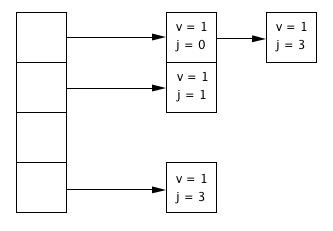
\includegraphics[width=7cm]{encodage.png}
		\caption{Encodage d'une matrice creuse par lignes}
		\label{encodage}
	\end{center}
\end{figure}


\subsection{Multiplication et multithreading}
Nous nous sommes ensuite rendu compte que nous pouvions rendre la multiplication de deux matrices creuses $A$ et $B$ plus aisée en encodant $A$ comme présenté ci-dessus mais en encodant $B$ à l'aide de la même structure de données mais en colonnes, c'est-à-dire que la $i^{ème}$ file du tableau représente la $i^{ème}$ colonne de la matrice et plus la $i^{ème}$ ligne. Nous avons donc rajouté un booléen dans notre structure de matrice creuse indiquant si notre matrice était encodée en lignes ou en colonnes. Notre matrice exemple serait alors encodée comme représenté à la Figure~\ref{encodage2}.\\

\begin{figure}[!!h]
	\begin{center}
		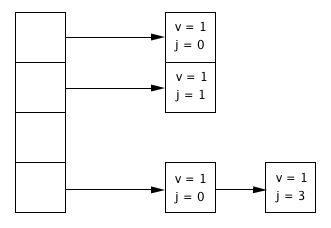
\includegraphics[width=7cm]{encodage2.png}
		\caption{Encodage d'une matrice creuse par colonnes}
		\label{encodage2}
	\end{center}
\end{figure}

Pour effectuer le produit d'un certain nombre de matrices creuses, c'est-à-dire calculer $$X = M_1 M_2 M_3 M_4 ... M_N$$
nous avons encodé notre matrice $M_1$ en lignes et toutes les autres en colonnes. Nous effectuons alors le produit de $(M_1 M_2)$ que nous encodons en lignes, puis le multiplions par $M_3$, etc.\\

Nous n'avons pas multithreadé notre programme mais si nous l'avions fait, nous aurions effectué le plus de produit du type $(M_1 M_2)$, $(M_3 M_4)$, $(M_5 M_6)$, ... en même temps en encodant les matrices d'indices pairs en colonnes. Le résultat de $(M_1 M_2)$ serait alors encodé en lignes, $(M_3 M_4)$ en colonnes, etc. Dans cette optique, nous avons permis de stipuler à la fonction effectuant le produit de deux matrices creuses si nous voulons que le résultat du produit soit encodé en lignes ou en colonnes, mais comme nous n'avons finalement pas multithreadé notre programme, nous l'utilisons exclusivement pour rendre un résultat en lignes. Notons toutefois que le programme en reste modulaire.

\subsection{Détails techniques}
Nous avons considéré que nos fichiers d'entrées contenaient des matrices du type\\
\texttt{
2x3\\
0 1 0 \\
1 0 1\\}
et que le fichier terminait par maximum un retour à la ligne. Si il y en a plus, nous cherchons une prochaine matrice.

\subsection{Valgrind}

Nous avons testé notre programme avec \texttt{Valgrind}. Notre seul problème est qu'il reste $33$ blocks ``still reachable''. Nous avons testé avec plusieurs fichiers d'entrée différents et ce nombre de 33 blocks semble constant. Le problème pourrait donc provenir de fonctions de la libraire standard que nous appelons.

\section{Mesures de performance et interprétations}

Il est intéressant d'analyser les performances de notre programme en comparaison avec une implémentation triviale des matrices pleines afin de voir dans quel cas il est intéressant de travailler avec des matrices creuses. Nous avons donc créé un deuxième programme qui effectue toutes les mêmes opérations mais en utilisant de simples tableaux à deux dimensions, et avons comparé les temps d'exécution des deux programmes sur un de nos ordinateurs personnels. Ils sont tous deux équipés d'un processeur Intel Core i5 de cadence horloge $1,7$ GHz et de $2$ c\oe urs. La mémoire est de taille $4$ Go.

\subsection{Scénario 1 : variation du nombre d'éléments non nuls}

Nous avons tout d'abord voulu analyser l'influence du nombre d'éléments non nuls sur le temps d'exécution. Nous avons pour cela généré des fichiers contenant deux fois une même matrice $1000$x$1000$ avec respectivement $1$, $3$, $9$, $27$, $81$ ou $243$ éléments non nuls par ligne (des $1$ en l'occurrence), décalés d'une ligne à l'autre afin d'éviter d'avoir des colonnes vides. Autrement dit, notre premier fichier contenait deux matrices identité de taille $1000$, notre deuxième fichier deux matrices de taille $1000$ aussi mais avec trois $1$ sur chaque ligne, etc. Nous avons ensuite calculé le temps d'exécution de nos deux programmes pour lire les deux matrices d'un fichier, les multiplier, et écrire le résultat dans un fichier de sortie. 

\paragraph{Mesures}
Afin d'éviter d'avoir des valeurs aberrantes, nous avons effectué 3 mesures dans chacune des situations. \\

\begin{tabular}{|*{7}{c|}}
    \hline
       & 1  & 3  & 9  & 27  & 81  & 243 \\
    \hline
    \multirow{3}{*}{creuses}  & 0.257357 s & 0.312883 s & 0.646042 s & 2.996151 s & 43.934574 s & 226.217773 s\\
    & 0.262014 s & 0.304584 s & 0.651323 s & 3.018808 s & 43.854031 s & 229.002350 s\\
    & 0.264037 s & 0.310822 s & 0.639835 s & 2.994909 s & 43.921665 s & 227.610432 s\\
    \hline
     \multirow{3}{*}{pleines} & 17.634382 s & 18.294992 s & 18.809765 s  & 19.883987 s & 18.096115 s & 18.203505 s\\
    & 18.027992 s & 20.234669 s & 18.161089 s & 20.196924 s & 18.096998 s & 18.051762 s\\
    & 21.453005 s & 18.225401 s & 18.242275 s & 18.125992 s & 18.777365 s & 20.237141 s\\
    \hline
\end{tabular}


\paragraph{Graphe}
Nous avons ensuite tracé un graphe logarithmique de ces résultats en utilisant les moyennes de ces 3 mesures dans chacun des cas (voir Figure~\ref{vnz}).
\begin{figure}[!h]
	\begin{center}
		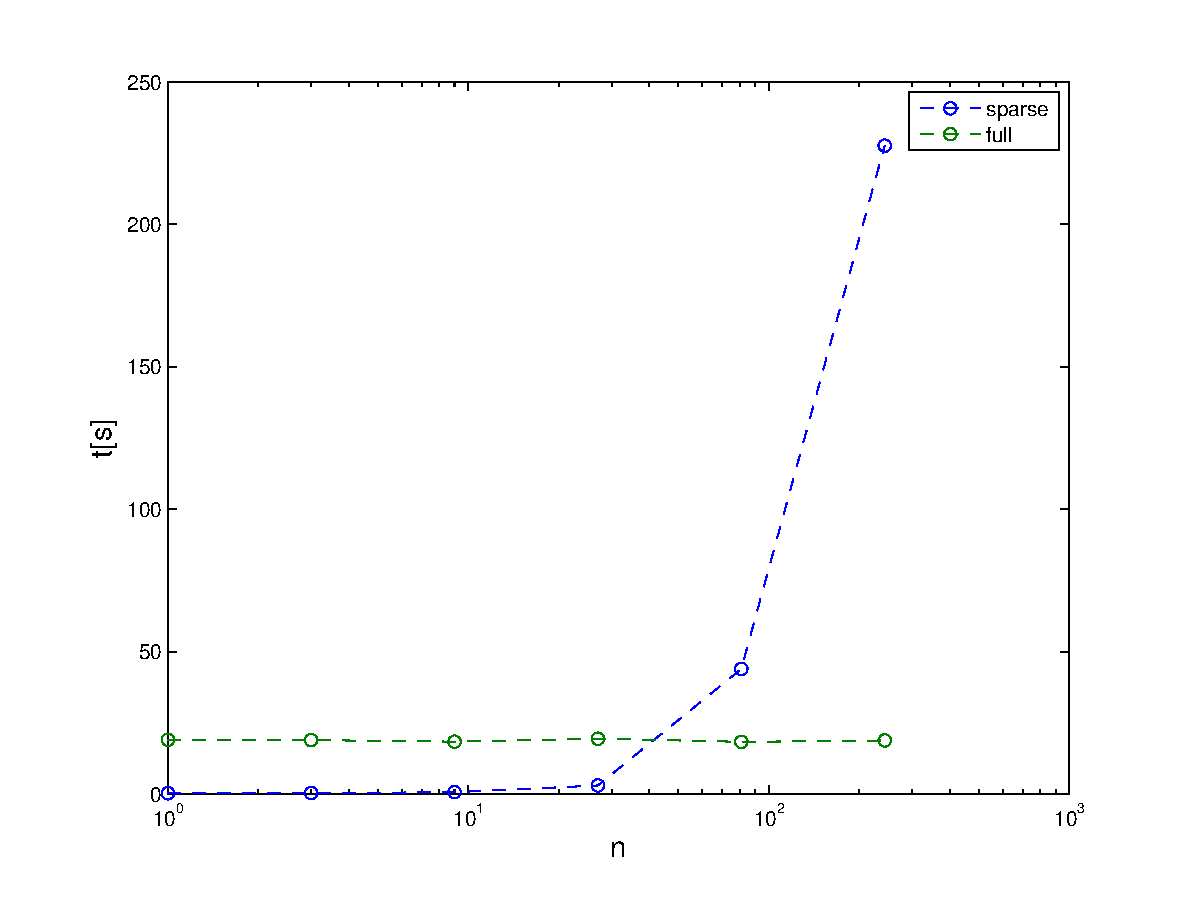
\includegraphics[width=15cm]{taillecst.eps}
		\caption{Scénario 1 : variation du nombre d'éléments non nuls}
		\label{vnz}
	\end{center}
\end{figure}

\paragraph{Observations}

On remarque tout d'abord que pour des matrices pleines, le temps d'exécution ne dépend pas du nombre d'éléments non nuls dans la matrice. Cela est tout à fait logique car on utilise un simple tableau qu'il faut de toutes façon parcourir dans son entièreté lorsqu'on veut le multiplier par une autre matrice. Pour des matrices creuses par contre, le nombre d'éléments non nuls a de l'influence car nos files vont alors avoir plus de noeuds qu'il va falloir parcourir pour effectuer un produit.\\

On remarque ensuite que jusqu'à 2,7\% d'éléments non nuls, il était nettement plus avantageux (environ $7$ fois plus rapide) d'utiliser des matrices creuses tandis que lorsqu'il y en avait 8,1\%, c'était environ $2,5$ fois plus lent. Nous avons alors effectué d'autres tests afin de trouver à partir de quel pourcentage d'éléments nuls il est plus intéressant d'utiliser des matrices creuses et nous avons trouvé 93\%.

\subsection{Scénario 2 : variation de la taille de la matrice}

Nous avons ensuite voulu voir si, outre le pourcentage d'éléments non nuls dans la matrice, la taille de celle-ci pouvait avoir de l'influence. Nous avons donc choisi de travailler avec des matrices à 93\% nulles pour lesquelles on avait des temps d'exécutions semblables lorsqu'elles étaient de taille 1000 et avons voulu voir si une des deux implémentations était proportionnellement plus favorable dans le cas des petites ou des grandes matrices.

\paragraph{Mesures}
Nous avons généré des matrices carrées de taille 100, 200, 400, 800 et 1600 à 93\% nulles. De nouveau, afin d'éviter d'avoir des valeurs aberrantes, nous avons effectué 3 mesures dans chacune des situations. \\

\begin{tabular}{|*{7}{c|}}
    \hline
       & 100  & 200  & 400  & 800  & 1600\\
    \hline
    \multirow{3}{*}{creuses}  & 0.007116  s & 0.049152  s & 0.526088  s & 7.161576  s & 111.793129 s\\
    & 0.007053 s & 0.049568 s & 0.527764 s & 7.169523 s & 112.597748 s\\
    & 0.007125  s & 0.049119 s &0.526721 s & 7.174552 s & 112.649086 s\\
    \hline
     \multirow{3}{*}{pleines} & 0.017462 s & 0.113815 s & 0.955724 s  &  8.053343 s & 75.238472 s\\
    & 0.015019 s & 0.111238 s & 0.931406 s & 8.676009 s & 74.620865 s\\
    & 0.015758 s & 0.115848 s & 0.950773 s & 8.642730 s & 74.007690 s\\
    \hline
\end{tabular}

\paragraph{Graphe}
Nous avons ensuite tracé le graphe (voir Figure~\ref{vtm}) du rapport entre le temps pris avec les matrices pleines et le temps pris avec les matrices creuses, en fonction de la taille de la matrice (échelle logarithmique).
\begin{figure}[!h]
	\begin{center}
		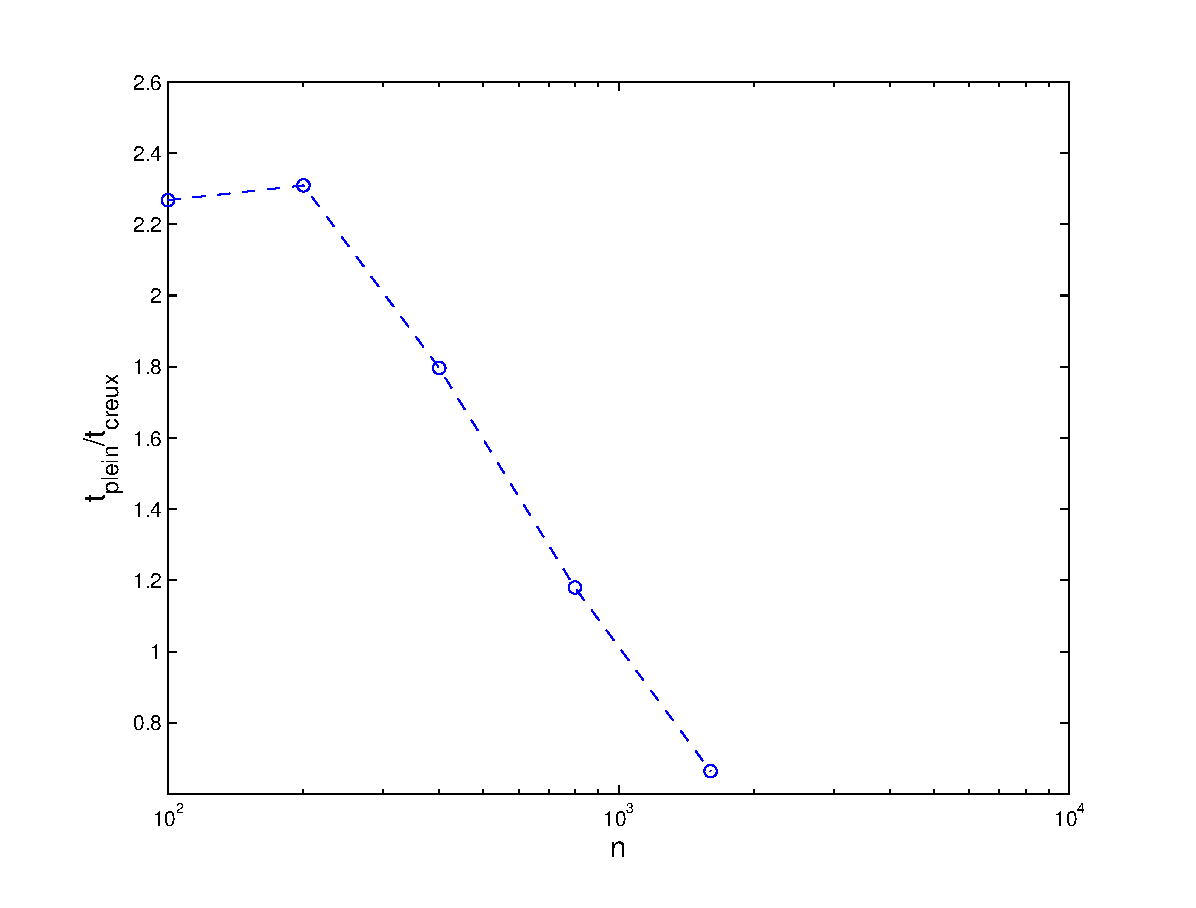
\includegraphics[width=15cm]{pourccst.eps}
		\caption{Scénario 2 : variation de la taille de la matrice}
		\label{vtm}
	\end{center}
\end{figure}

\paragraph{Observations}
Globalement, il est intéressant d'utiliser des matrices creuses lorsque les matrices ne sont pas trop grandes (et on remarque bien qu'on a égalité vers une taille de 1000, ce qui confirme ce que l'on avait dit au point précédent). Plus celles-ci seront grandes, plus il faudra qu'elles aient un grand pourcentage d'éléments nuls pour que cela devienne intéressant. 

\subsection{Fichier de test fourni}
Notre programme prend environ $86$ minutes pour multiplier les matrices du fichier de test fourni, versus $23$ minutes avec une implémentation basique de matrices pleines. Cela est dû au fait qu'après multiplications, on se retrouve avec des matrices de moins en moins creuses. Le résultat final ne contient d'ailleurs plus aucun zéro.

%\section{Performances}
%\subsection{Fonctionnement}
%\subsection{Comparaison avec une implémentation triviale de matrices pleines}
%\subsection{Domaines d'application}
%
%\section{Mesures}
%\subsection{Spécifications}
%\subsection{Résultat}
%\subsection{Interprétation}

\end{document}